% Metódy inžinierskej práce

\documentclass[10pt,slovak,a4paper]{article}

\usepackage[slovak]{babel}
%\usepackage[T1]{fontenc}
\usepackage[IL2]{fontenc} % lepšia sadzba písmena Ľ než v T1
\usepackage[utf8]{inputenc}
\usepackage{graphicx}
\usepackage{url} % príkaz \url na formátovanie URL
\usepackage{hyperref} % odkazy v texte budú aktívne (pri niektorých triedach dokumentov spôsobuje posun textu)

\usepackage{cite}
%\usepackage{times}

\pagestyle{plain}

\title{Sekvenčné UML Diagramy\thanks{Semestrálny projekt v predmete Metódy inžinierskej práce, ak. rok 2021/22, vedenie: Ing. Ján Lúčanský}}

\author{Kristián Lukacsovics\\[2pt]
    {\small Slovenská technická univerzita v Bratislave}\\
    {\small Fakulta informatiky a informačných technológií}\\
    {\small \texttt{xlukacsovics@stuba.sk}}
    }

\date{\small 14.12.2021} % upravte

\providecommand{\abstr}[1]{\textbf{\textit{Abstrakt---}} #1}
\providecommand{\keywords}[1]{\textbf{\textit{Klúčové slová---}} #1}

\begin{document}

\maketitle

\abstr{Tento článok sa zameriava na opis sekvenčných UML diagramov\ldots\newline}
\indent\keywords{Unified Modeling Language, Sekvenčný diagram, Objekt, Správa}

\section{Úvod}
UML, celým názvom Unified Modeling Language, je objektovo-orientovaný modelovací jazyk pre softvérové programy. \cite{eriksson98}
Existuje niekoľko typov UML diagramov, sekvenčné diagramy sú jedným z nich. Všetky tieto diagramy slúžia na
abstraktný opis správania sa jednotlivých častí počítačového programu. Každý jeden typ sa sústreďuje na opis
rôznych vlastností kódu. Cieľom sekvenčných diagramov je opis interakcie medzi objektami programu, s tým, že sa
berie ohľad na poradie vykonávaného postupu. \cite{petraq14}

\section{Úroveň využitia}
Lorem ipsum dolor sit amet, consectetur adipiscing elit. Sed pellentesque pretium urna, non convallis ante consequat nec. 
Quisque nec tellus a est ornare hendrerit eu vel nisl. Sed aliquet augue nisi, in porttitor urna ultrices sed. 
Aliquam ultrices sagittis quam ut maximus. Sed rutrum, dui vitae pulvinar convallis, ex odio maximus justo, id finibus ligula turpis non elit. 
Cras imperdiet finibus augue vel fermentum. Maecenas ac nibh ullamcorper, tempor magna et, congue elit. \newline

Lorem ipsum dolor sit amet, consectetur adipiscing elit. Sed pellentesque pretium urna, non convallis ante consequat nec. 
Quisque nec tellus a est ornare hendrerit eu vel nisl. Sed aliquet augue nisi, in porttitor urna ultrices sed.
Aliquam ultrices sagittis quam ut maximus. Sed rutrum, dui vitae pulvinar convallis, ex odio maximus justo, id finibus ligula turpis non elit. 
Cras imperdiet finibus augue vel fermentum. Maecenas ac nibh ullamcorper, tempor magna et, congue elit.

\begin{figure*}[tbh]
\centering
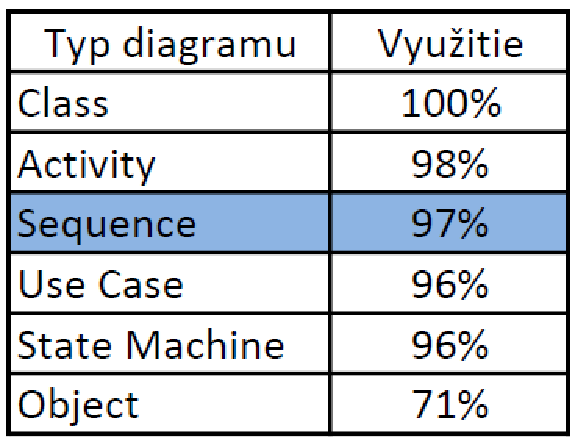
\includegraphics[scale=0.5]{tab.pdf}
\caption{Úroveň využitia jednotlivých typov UML diagramov. \cite{reggio13}}
\end{figure*}

\section{Komunikácia objektov}

\noindent Objekty si navzájom posielajú správy (požiadavky) medzi sebou. Tieto
správy medzi objektami sa v diagrame zaznačia ako horizontálne šípky. Smer týchto šípok určuje odosielateľa a
príjemcu (na strane, kde je šípka, je príjemca). Samotné objekty sa značia ako vertikálne čiary, s tým, že
na vrchu tejto čiary je meno objektu. Tieto vertikálne čiary značia aj dĺžku života objektov. Úseky, kde sú
čiary prerušované, značia časové úseky programu, kde dané objekty ešte neboli vytvorené, resp. už boli odstránené. \newline

\noindent Objekty si môžu poslať správy aj pre seba. Takéto správy sa nazývajú reflexívne správy. 
Ako už bolo spomenuté, poradie týchto správ je dôležité. Zmena poradia môže zmeniť korektnosť programu
v niektorých prípadoch. \cite{petraq14}

%\noindent Na obr. 2 môžeme vidieť veľmi jednoduchú ukážku sekvenčného UML diagramu.

\begin{figure*}[tbh]
\centering
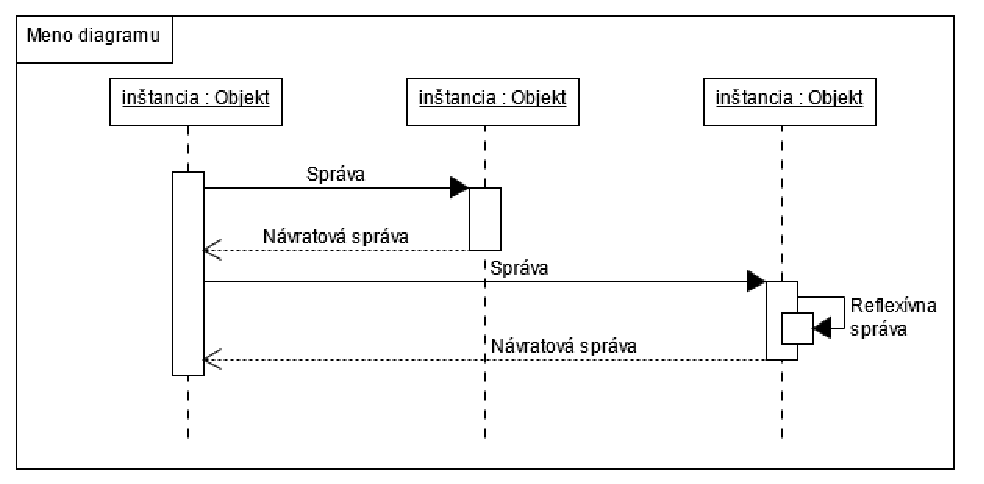
\includegraphics[scale=0.8]{simple_diag.pdf}
\caption{Ukážka sekvenčného diagramu.\cite{booch00}}
\end{figure*}

\section{Ďalšia časť}

Lorem ipsum dolor sit amet, consectetur adipiscing elit. Sed pellentesque pretium urna, non convallis ante consequat nec. 
Quisque nec tellus a est ornare hendrerit eu vel nisl. Sed aliquet augue nisi, in porttitor urna ultrices sed.
Aliquam ultrices sagittis quam ut maximus. Sed rutrum, dui vitae pulvinar convallis, ex odio maximus justo, id finibus ligula turpis non elit. 
Cras imperdiet finibus augue vel fermentum. Maecenas ac nibh ullamcorper, tempor magna et, congue elit.

\begin{figure*}[tbh]
\centering
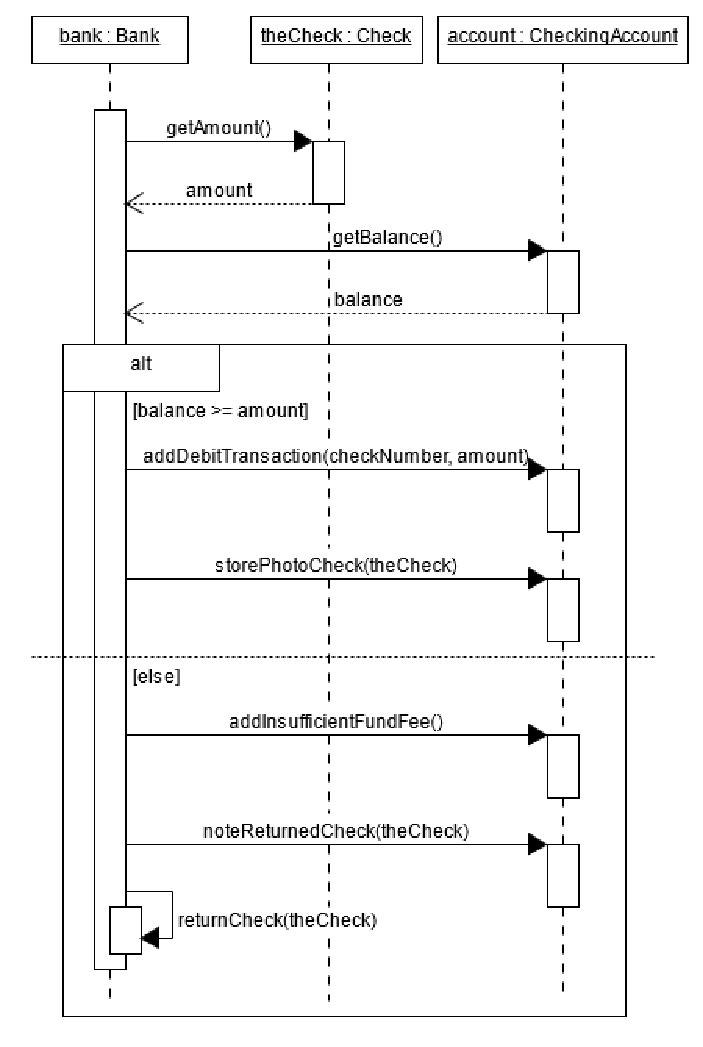
\includegraphics[scale=0.8]{cond_diag.pdf}
\caption{Modelovanie podmienok. \cite{booch00}}
\end{figure*}

\section{Záver}
\ldots

%\acknowledgement{Ak niekomu chcete poďakovať\ldots}


% týmto sa generuje zoznam literatúry z obsahu súboru literature.bib podľa toho, na čo sa v článku odkazujete
\bibliography{literature}
\bibliographystyle{plain} % prípadne alpha, abbrv alebo hociktorý iný
\end{document}
